\section{Evaluation}
\label{sec:liveclips_eval}
To evaluate whether our ranking metrics are effective at finding inspiring clips, we conducted a study on Amazon Mechanical Turk. This study did not evaluate clips in the context of creative software. Instead, it focused on whether timing and visual change are good general predictors for inspiring content. 

As described in the System section, LiveClips generated 1,742 clips from our dataset of 30 hours of video of Photoshop and Illustrator use. We randomly sampled 129 of these clips to include in our evaluation set. To ensure we had coverage of all tools in our dataset, we randomly chose between 2 and 10 clips per tool. Since some tools are much more popular than others (\textit{e.g.}, Photoshop's brush tool had 939 clips whereas the burn tool only had 2 clips), this method allowed us to have a smaller sample while still representing every tool.

\begin{figure}[t!]
\centering
  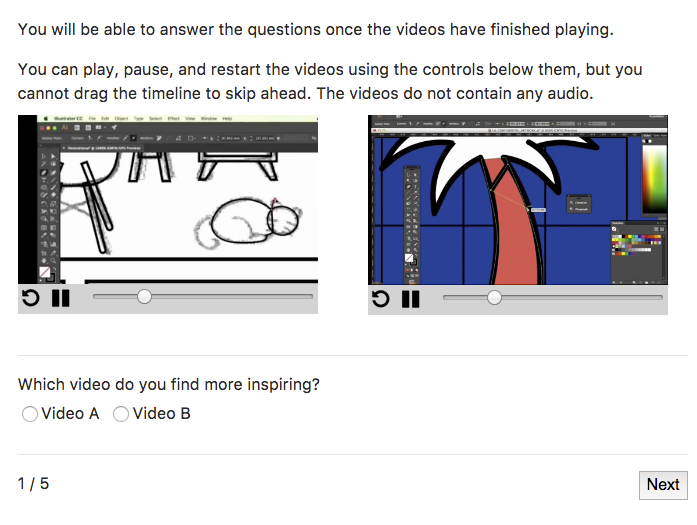
\includegraphics[width=0.8\columnwidth]{liveclips/figures/mturk.png}
  \caption{An example of a pairwise comparison completed by Mechanical Turk workers. Each task involved five such pairs. In the introduction to the task, workers were asked to consider which 25-second video would inspire them to be more creative. }~\label{fig:liveclips_mturk}
\end{figure}

Workers compared video clips in pairs. Each Mechanical Turk task started with an overview page describing the task and showing an example pair of clips followed by five rounds of paired comparisons. Each comparison involved viewing two clips of the same tool and answering which clip they think would inspire them to be more creative (\autoref{fig:liveclips_mturk}). After completing all five comparisons, workers completed a short survey asking about their experience with Photoshop and Illustrator, and what types of creative tasks they do. Workers' results were only included if they completed all of the above steps. In an effort to ensure that they actually watched the videos, each comparison page only allowed workers to answer the question once both videos had played through once. Workers were paid \$1.50 per task, which took an average of 10 minutes and 20 seconds to complete. The same worker could do multiple tasks and would see five new pairs of videos (randomly selected) every time.

\subsection{Results}
In total, 481 workers completed 628 tasks, giving us a total of 3,140 paired comparisons. Most pairs were compared by 9 unique workers, though some ended up being compared more times. To balance results across clips, we considered only the first 9 comparisons for each pair. \autoref{table:liveclips_experience} shows the distribution of workers' prior experience with Photoshop, Illustrator, and various types of creative tasks. Notably, 73\% and 35\% of participants had at least some experience using Photoshop and Illustrator respectively.

\begin{table}[t!]
\small
\centering
\caption{The distribution of workers' experience with Photoshop and Illustrator, and the types of creative tasks they have experience with.}
\label{table:liveclips_experience}
\begin{tabular}{lll}
            &                           & \# Participants \\ \hline
Photoshop   & None                      & 130 (27\%)       \\
experience  & Beginner                  & 242 (50\%)      \\
            & Intermediate              & 91 (19\%)       \\
            & Expert                    & 18 (4\%)        \\ \hline
Illustrator & None                      & 311 (65\%)      \\
experience  & Beginner                  & 114 (24\%)      \\
            & Intermediate              & 46 (9\%)       \\
            & Expert                    & 10 (2\%)        \\ \hline
Creative    & Physical drawing/painting & 247 (51\%)      \\
experience  & Digital drawing/painting  & 147 (31\%)      \\
            & Photography               & 386 (80\%)      \\
            & Photo editing             & 290 (60\%)      \\
            & Design                    & 144 (30\%)     
\end{tabular}
\end{table}

Since only clips showing the same tool were compared, our analysis only examines ranking agreement within tool groups. Each tool group had between 2 and 10 video clips. For groups with only 2 clips, we determine the human ranking of these two clips by ranking whichever clip was chosen more often first, and the other second. For all other groups, we use the Bradley-Terry model as implemented in \cite{Maystre2015} to infer a ranking of clips within that group based on the paired comparisons. Within each group, we use Spearman's $\rho$ to compute the correlation between human rankings and LiveClips rankings. LiveClips rankings are based on the total score for each clip (time and visual change combined).

\textbf{Overall agreement between rankings ranges between very weak and moderate.} Since the groups have different sizes, we cannot compute one overall measure of correlation, as it is unclear what the null distribution would be. \autoref{table:liveclips_agreement} (top) shows the average $\rho$ values for each group size. Note that $p$-values are not appropriate for such small group sizes, however the $\rho$ values still accurately represent the correlation between rankings. \autoref{fig:liveclips_agreement} (left) shows an aggregate comparison of all clip rankings. 

\begin{table}[t!]
\small
\centering
\caption[Average Spearman $\rho$ correlation between human ranking and LiveClips ranking for all clips (top) and all clips with >65\% agreement among turkers (bottom), compared within each tool.]{Average Spearman $\rho$ correlation between human ranking and LiveClips ranking for all clips (top) and all clips with >65\% agreement among turkers (bottom), compared within each tool. ``\# Groups'' for column $i$ refers to the number of tools that have $i$ clips. Positive $\rho$ values indicate a positive correlation, with correlations above .2 considered weak, above .4 considered moderate, and above .6 considered strong.}
\label{table:liveclips_agreement}
\textbf{All clips (n = 115)}\\
\vspace{5pt}
\begin{tabular}{l|llllllll}
\# Clips & 2    & 3 & 4 & 5   & 6    & 7    & 9    & 10   \\ \hline
\# Groups           & 18   & 5 & 2 & 1   & 1    & 1    & 2    & 2    \\
Mean $\rho$  & 0.11 & 0.3 & -0.2 & 0.6 & 0.09 & 0.54 & 0.21 & 0.48
\end{tabular}\\
\vspace{5pt}
\textbf{Clips with >65\% agreement (n = 64)}\\
\vspace{5pt}
\begin{tabular}{l|llll}
\# Clips & 2    & 3   & 4    & 5   \\ \hline
\# Groups           & 18   & 3   & 3    & 1   \\
Mean $\rho$  & 0.33 & 1.0 & 0.73 & 1.0
\end{tabular}
\end{table}

\begin{figure}[t!]
\centering
  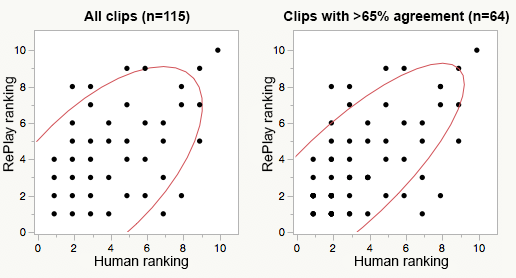
\includegraphics[width=0.65\columnwidth]{liveclips/figures/agreement.png}
  \caption{Human ranking vs. LiveClips ranking for all video clips (left), and all video clips with >65\% agreement among turkers (right). Note that there is more overall agreement between rankings in the subset on the right.}~\label{fig:liveclips_agreement}
\end{figure}


\textbf{Agreement between rankings for less-disputed clips ranges between weak and very strong.} The main goal of LiveClips' ranking is not to establish an overall ranking of \textit{all} clips, but rather to ensure that bad clips are discarded, and that only the best clips are shown to the user. Therefore, any clips that had a large amount of disagreement between workers are likely not among the best. Indeed, if we restrict our selection of video clips to only those that either won or lost over 65\% of all comparisons they were a part of, this set consists of video clips that likely have a more obvious objective value. \autoref{table:liveclips_agreement} (bottom) shows the average $\rho$ values for each group size when restricted to this smaller set of clips (in our sample set, 64/115). Overall we see stronger correlations. \autoref{fig:liveclips_agreement} (right) shows an aggregate comparison of all these clips' rankings; we see fewer large disagreements here than in \autoref{fig:liveclips_agreement} (left).

Timelapse clips did not perform significantly better or worse than standard clips. However, there were far fewer timelapse clips than standard ones in our dataset (19 vs. 96), due to the fact that longer sequences of a single tool use were less common overall than shorter sequences. A larger dataset is needed to determine whether or not timelapse videos may be preferred over standard ones.

\section{Early User Feedback}
The Mechanical Turk evaluation explored the viability of LiveClips' ranking algorithm outside the context of an application. To get some initial user feedback on placing inspiring examples \textit{inside} an application, we recruited two casual Photoshop users, both male, to work on projects of their choice. They used Photoshop with all three interfaces enabled at once (on-demand search, ambient side panel, and contextual tooltips) (\autoref{fig:liveclips_photoshop}), and gave feedback while they worked.

Overall feedback was positive. Both participants found seeing video examples in the application useful and said that they wanted to see how others use tools and set parameters. The two participants differed in how they wanted to see examples. One participant preferred the tooltips, explaining that they were a nice level in between the on-demand search (which was easy to forget about) and the ambient panel (which they found distracting). They liked that if you happen to hover on a tool for an extra moment (which could happen by accident), it pops up and serves as a reminder that these examples exist, without taking away too much from the process. The other participant preferred the panel, and wanted to be able to refresh recommendations on demand and see a large variety of content. Both participants clicked on the videos and wanted to watch them in the browser where they could see them larger. 

This early user feedback is encouraging and shows the opportunity around embedding inspirational examples in creative software.

